\documentclass[a4paper,10pt]{article}
\usepackage{asp2014}
\usepackage[utf8]{inputenc}

\aspSuppressVolSlug
\resetcounters

\bibliographystyle{asp2014}

\markboth{Author1, Author2, and Author3}{Sort Last Screen Space Surface LIC}

\begin{document}
\title{A Screen Space GPGPU Surface LIC Algorithm for Distributed Memory Data Parallel Sort Last Rendering Infrastructures}
\author{B. Loring,$^1$ H. Karimabadi,$^2$ and V. Rortershteyn$^2$
\affil{\small $^1$Lawrence Berkeley Laboratory, Berkeley, California, USA; \email{bloring@lbl.gov}}
\affil{\small $^2$Department of Electrical and Computer Engineering, University of California, San Diego, USA; \email{homakar@gmail.com}}}
%\affil{$^3$Department of Electrical and Computer Engineering, University of California, San Diego, USA; \email{vroytersh@gmail.com}}}
%W. Daughton, Los Alamos National Laboratory, USA

% This section is for ADS Processing.  There must be one line per author.
\paperauthor{B. Loring}{bloring@lbl.gov}{}{Lawrence Berkeley Laboratory}{CRD}{Berkeley}{CA}{94720}{USA}
\paperauthor{H. Karimabadi}{homakar@gmail.com}{}{University of California, San Diego}{ECE}{San Diego}{CA}{92093}{USA}
\paperauthor{V. Rortershteyn}{vroytersh@gmail.com}{}{University of California, San Diego}{ECE}{San Diego}{CA}{92093}{USA}

\begin{abstract}
The surface line integral convolution(LIC) visualization technique produces dense visualization of vector fields on arbitrary surfaces. We present a screen space surface LIC algorithm for use in distributed memory data parallel sort last rendering infrastructures. The motivations for our work are to support analysis of datasets that are too large to fit in the main memory of a single computer and compatibility with prevalent parallel scientific visualization tools such as ParaView and VisIt. By working in screen space using OpenGL we can leverage the computational power of GPUs when they are available and run without them when they are not. We address efficiency and performance issues that arise from the transformation of data from physical to screen space by selecting an alternate screen space domain decomposition. We analyze the algorithm's scaling behavior with and without GPUs on two high performance computing systems using data from turbulent plasma simulations.
\end{abstract}

\section{Introduction}
The line integral convolution is a technique for producing dense visualizations of vector fields. The technique works by convolving a noise texture along vector field streamlines to produce streaks of varying intensity. The original LIC algorithm\citep{lic} was designed for use on images. A two pass method was introduced to address the algorithm's inherent dynamic range truncation and resulting low contrast streaks\citep{elic}. The image LIC algorithm was later extended to arbitrary geometric surfaces\citep{surflic} followed by the development of screen space algorithm\citep{gpulic} that allowed the computational power of GPUs to be utilized. The screen space algorithm has been parallelized for use on clusters of GPUs using a hybrid sort-first sort-last algorithm\citep{pargpulic}. However, the necessity of duplicating vector and geometric data on all nodes in the hybrid sort-first sort-last approach limits its applicability to relatively small datasets and is incompatible with popular scientific data visualization frameworks which are based on a distributed memory data parallel  sort-last rendering(DMDPSLR) approach. VisIt \citep{visit} and ParaView \citep{paraview} are two examples of popular DMDPSLR based frameworks. In both tools the parallel sort-last rendering infrastructure is provided by IceT\citep{icet}, a highly optimized distributed memory data parallel image compositing library.

Here we introduce a parallel screen space GPGPU surface LIC algorithm targeted for use in DMDPSLR based frameworks on arbitrarily large scientific datasets. The motivations for our work are to support the processing of very large scientific datasets, specifically those which are too large to fit in the memory of a single computer, and compatibility with existing sort-last rendering frameworks. The screen space algorithm is implemented as part of the rendering pipeline using OpenGL and therefore can take advantage of the computational power of GPUs where they are available. The very same code can be run without GPUs by using a software based OpenGL implementation which is an important feature as many high-performance computing(HPC) systems do not have GPUs. This work has been integrated into ParaView.

\section{Parallelization}
\subsection{Distributed Memory Data Parallel Sort-Last Rendering}
\label{sec:DMDPSLR}
\begin{figure}
 \centering
 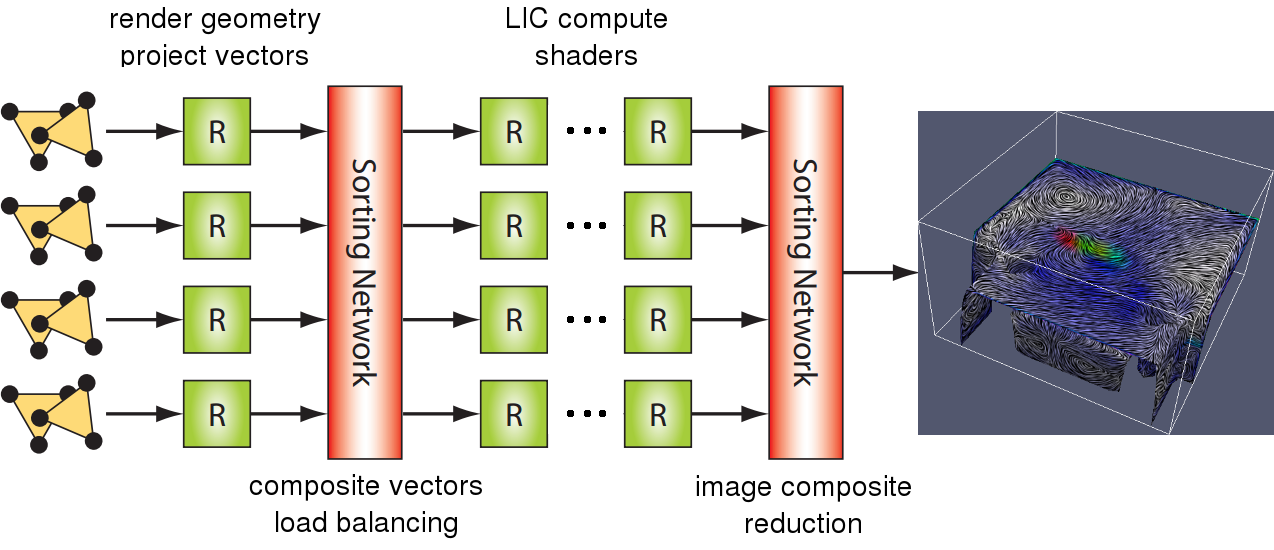
\includegraphics[width=0.7\textwidth]{render-sorting-plus-lic.png}
 % render-sorting.png: 738x550 pixel, 101dpi, 18.56x13.83 cm, bb=0 0 526 392
 \caption{Screen space surface LIC in a DMDPSLR setting is comprised of a sequence of local rendering(blocks) and global sorting operations(vertical bars). During parallel execution a sorting stage is needed during screen space transformation of vector data. See section \ref{sec:DMDPSLR}.}
 \label{fig:slr}
\end{figure}
Typically the sort-last rendering can be thought of as occurring in two main phases. The first phase contains a series of local graphics operations specific to the rendering algorithm. The second phase, called image compositing, exchanges and combines local renderings using a sorting algorithm into a single image on one process for display. The screen space surface LIC is atypical in that there are two sorting phases requiring inter-process communication with multiple purely local rendering operations intermixed. The first sort phase occurs during the transformation of vector data into screen space where overlapping regions of the screen space are exchanged and depth composited. The second sort phase performs the traditional image compositing reduction.

This is depicted in figure \ref{fig:slr}. Local graphics operations are represented by blocks while sorting operations requiring inter-process communication are represented by vertical bars. A vector field associated with surface geometry is input, a rendering stage transforms the vectors into screen space and performs surface rendering, a compositing stage then corrects the vector field in overlapping regions of the screen, a number of subsequent rendering stages compute the LIC in screen space, apply image processing filters, and combine the LIC with a pseduocolor plot, followed by the traditional image compositing stage that reduces locally rendered images into the final result on a single process for viewing. 

\begin{figure}
 \centering
 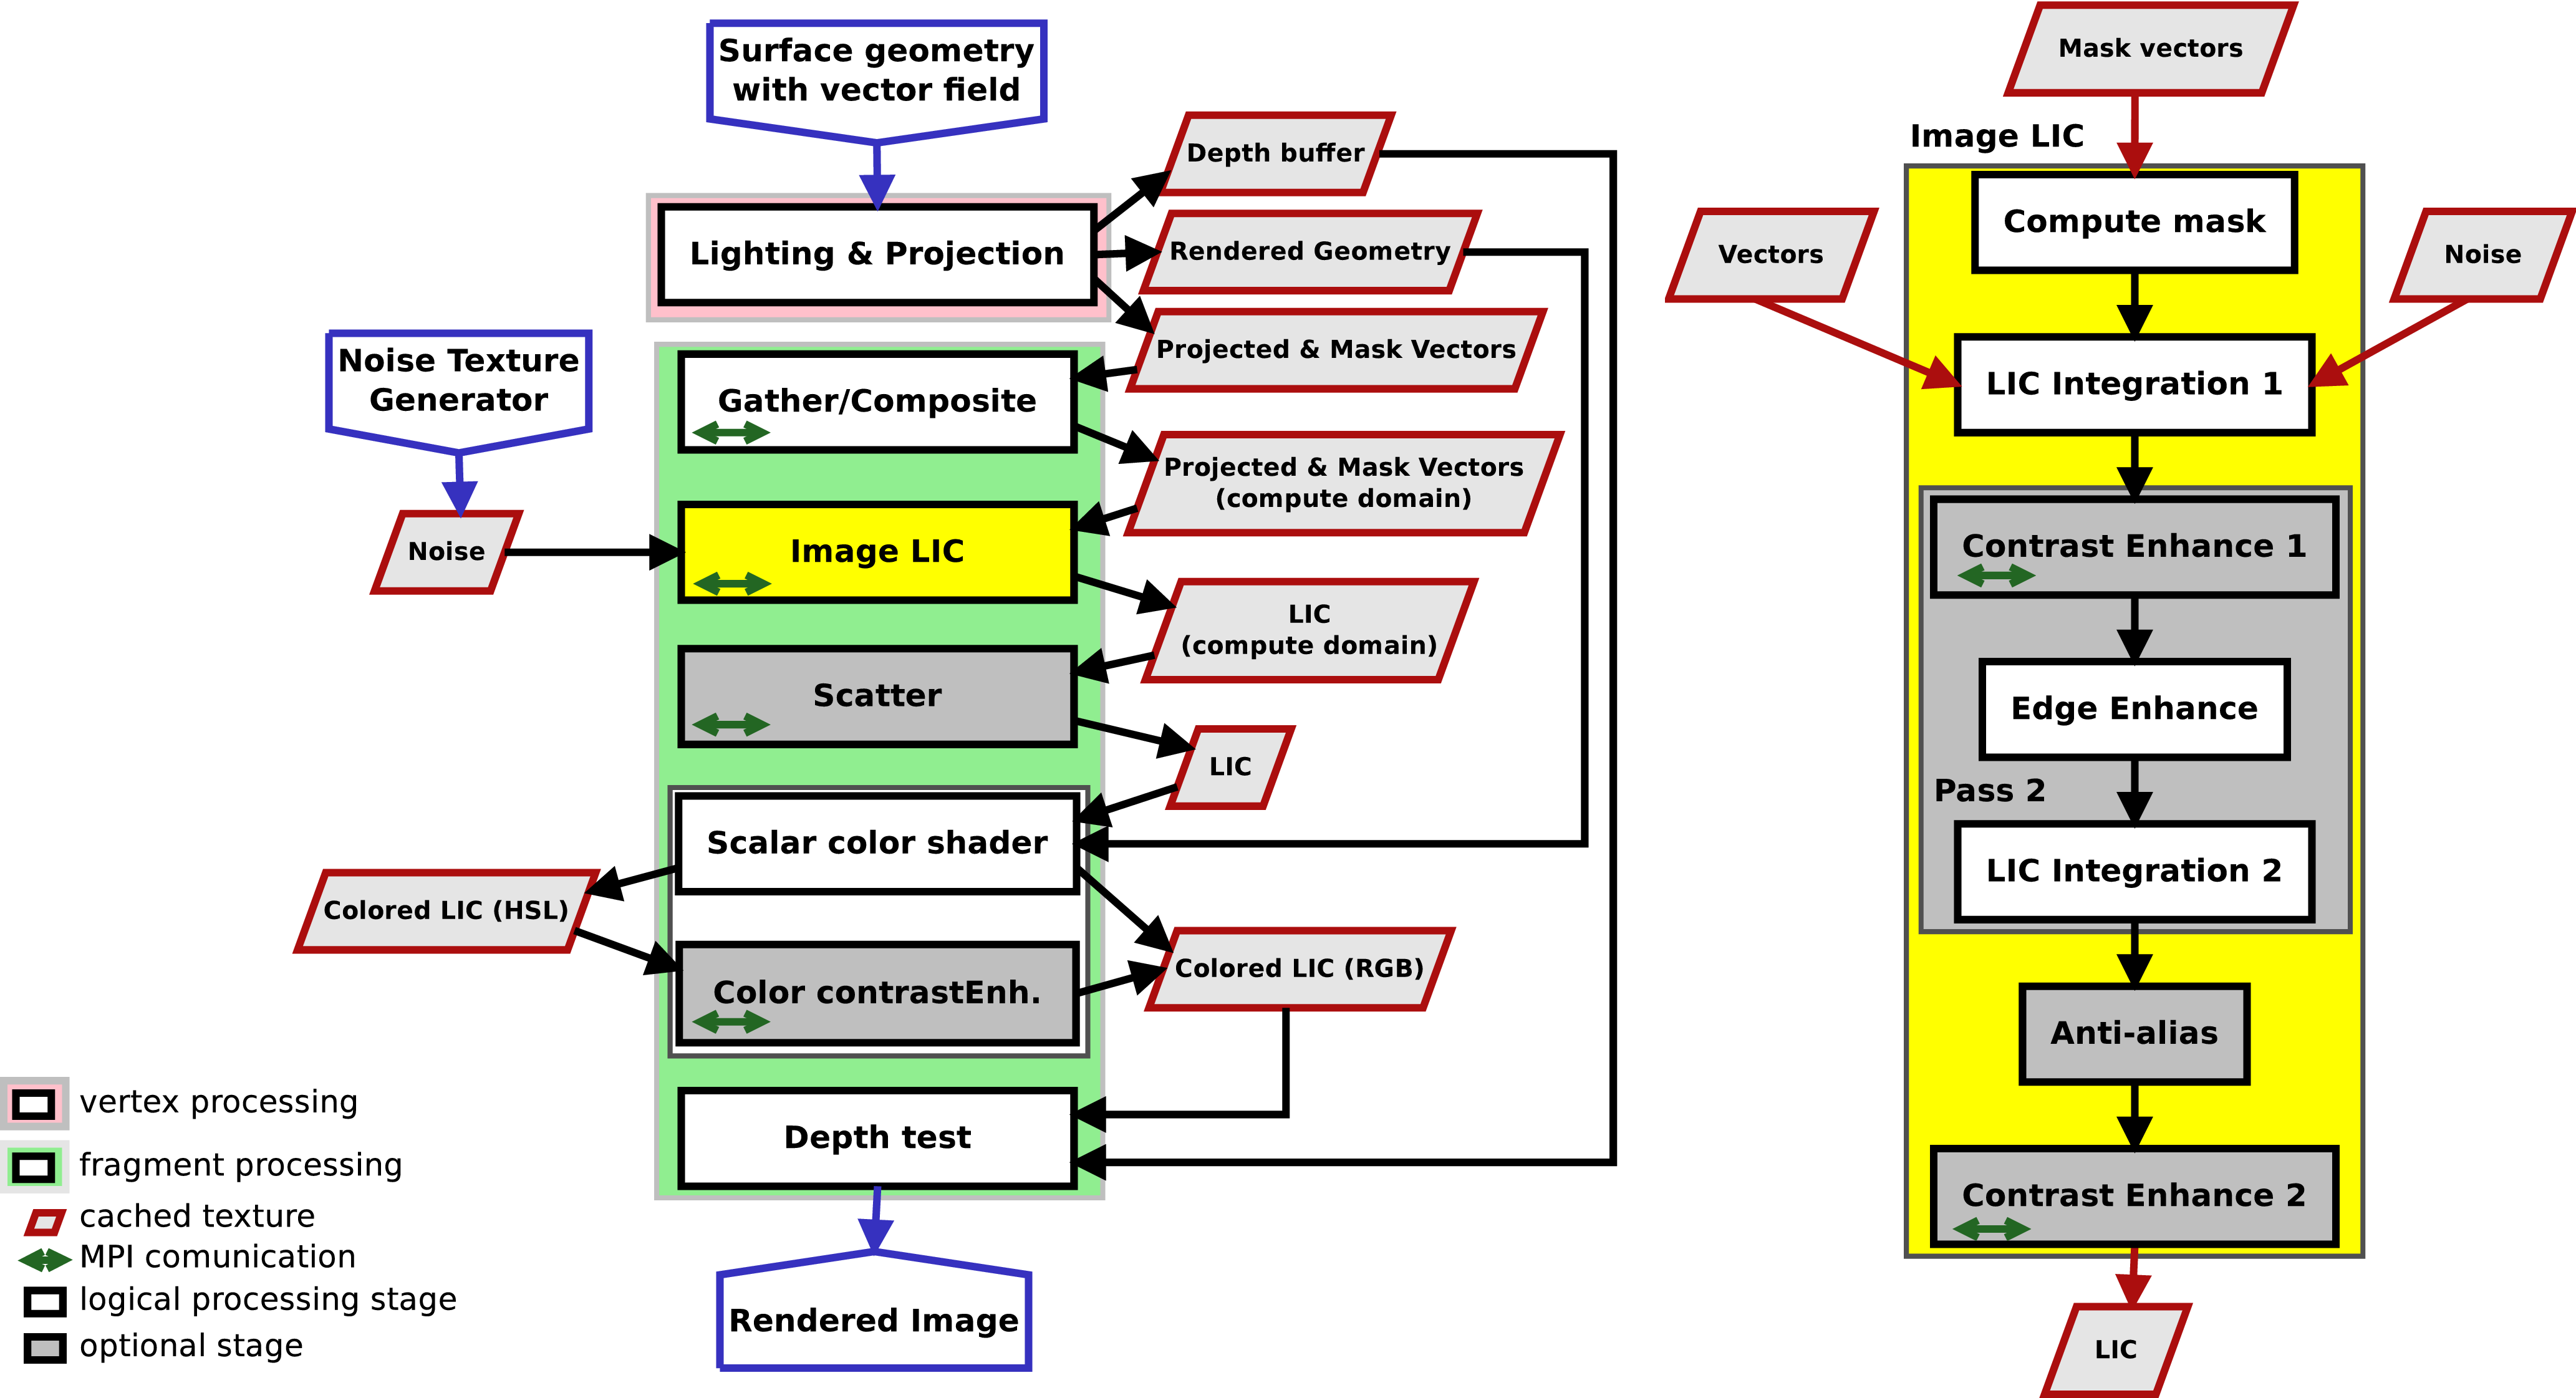
\includegraphics[height=2.8in]{flow-color.png}
 % flow-color.png: 4131x2242 pixel, 200dpi, 52.46x28.47 cm, bb=0 0 1487 807
 \caption{\small Pipeline. Left: Stages of the DPDMSLR screen surface LIC. Right: Breakout showing the two pass image LIC stage in detail.}
 \label{fig:pipeline}
\end{figure}
A high level schematic of our algorithm is shown in the left half of figure \ref{fig:pipeline} with the image LIC stage shown in detail on the right. We have organized the algorithm as a sequential pipeline to deliver high performance in an interactive setting. The result of each stage is cached and will be re-used during interaction if neither that stage's inputs nor its control parameters have been modified. In the following sections we describe the parallelization of the stages of our pipeline.

\subsection{Moving Vectors to Screen Space}
To obtain the correct vector field in screen space during parallel execution as the vector data is transformed into screen space it needs to be exchanged and depth buffer composited where there is off-process overlap in screen space. This occurs in the gather/composite stage of the pipeline in figure \ref{fig:pipeline}. To locate the overlapping regions we first gather a list of screen space extents on all processes. Extents, a light weight data structure describing a region in screen space coordinates, are obtained by projecting the axis aligned bounding box for each block of data to be rendered. The collection of extents organized by process id constitutes the screen space domain decomposition upon which the LIC will be computed. Each process maintains a copy of this list and uses it to coordinate inter-process communication and steer computation as the rendering pipeline executes.

Once all processes have the list of extents organized by process id each can determine the communication necessary for the required point to point exchange of vector data. These exchanges include filling the guard pixel halos required for correct parallel computation. We use non-blocking communication operations so that communication can be overlapped with compositing of incoming data. We use GPU mapped memory for communication buffers to minimize memory overhead.

\subsection{LIC Computation}
We used a two pass image LIC\citep{elic} with contrast enhancement(CE) stages to counteract inherent dynamic range reduction. Our CE stages are based on histogram normalization rather than equalization as the former is less costly to compute in parallel. We found that applying a CE stage on the L channel in HSL color space after the LIC is combined with pseudo-color plots generally increases dynamic range and improves perception of subtle color variations in the pseudo-coloring. We included an anti-aliasing filter to remove some of the jagged pixelation in LIC streaks that the high-pass edge enhancing filter tends to introduce. The organization of these stages are shown on the right in figure \ref{fig:pipeline}.

When executed in parallel the CE stages require the computation of the global minimum and maximum intensities. This requires the min and max values to be fetched from the GPU and a reduction applied across all processes. When executed in parallel the LIC integration, edge enhancement, and anti-aliasing stages all require some number of guard pixels to produce correct results. To eliminate the need for intermediate guard pixel exchanges, which in addition to communication overhead necessitates moving data on and off from the GPU, we precompute the total number of guard pixels required for all stages. The exchanges that fill the halos are made at the same time vector are composited in the gather/composite stage. Subsequent computations are nested such that upstream stages compute the solution in down stream stage's guard pixels. This avoids moving data on and off the GPU for communication at a slight increase in compositing and computation costs.

The anti-alias and edge enhancement stages are implemented with convolutions and require $\lfloor r/2 \rfloor$ guard pixels where $r$ is the convolution radius. For the LIC computation the number of guard pixels required on a given extent is a function of the local vector field. We use the maximum magnitude of the vector field on each extent to ensure we have a sufficient number of guard pixels. We need to add the guard pixel halos prior to compositing, but on any given screen space extent the vector field is not correct until after compositing. This requires us to search for the maximum vector magnitude in both the extent under consideration and in overlapping regions of off process extents as well. The number of guard pixels for a given extent is given by
\begin{equation}
  g(S_{i}) = \textrm{maxv}(S_{i}) \cdot n_s \cdot d_s \cdot n_p + n_{ee} + n_{aa}
\label{eqn:gaurd}
\end{equation}
where $S_i$ is one of the screen space extents, $\textrm{maxv}$ is a function that computes maximum vector magnitude across the extent and all overlapping regions of other extents, $d_s$ is the screen-space integration step size, $n_s$ is the number of integration steps, $n_p$ is the number of LIC passes, $n_{ee}$ and $n_{aa}$ are the number of guard pixels required for edge enhancement and anti-alias stages.

\subsection{Screen Space Domain Decomposition}
\begin{figure}
 \centering
 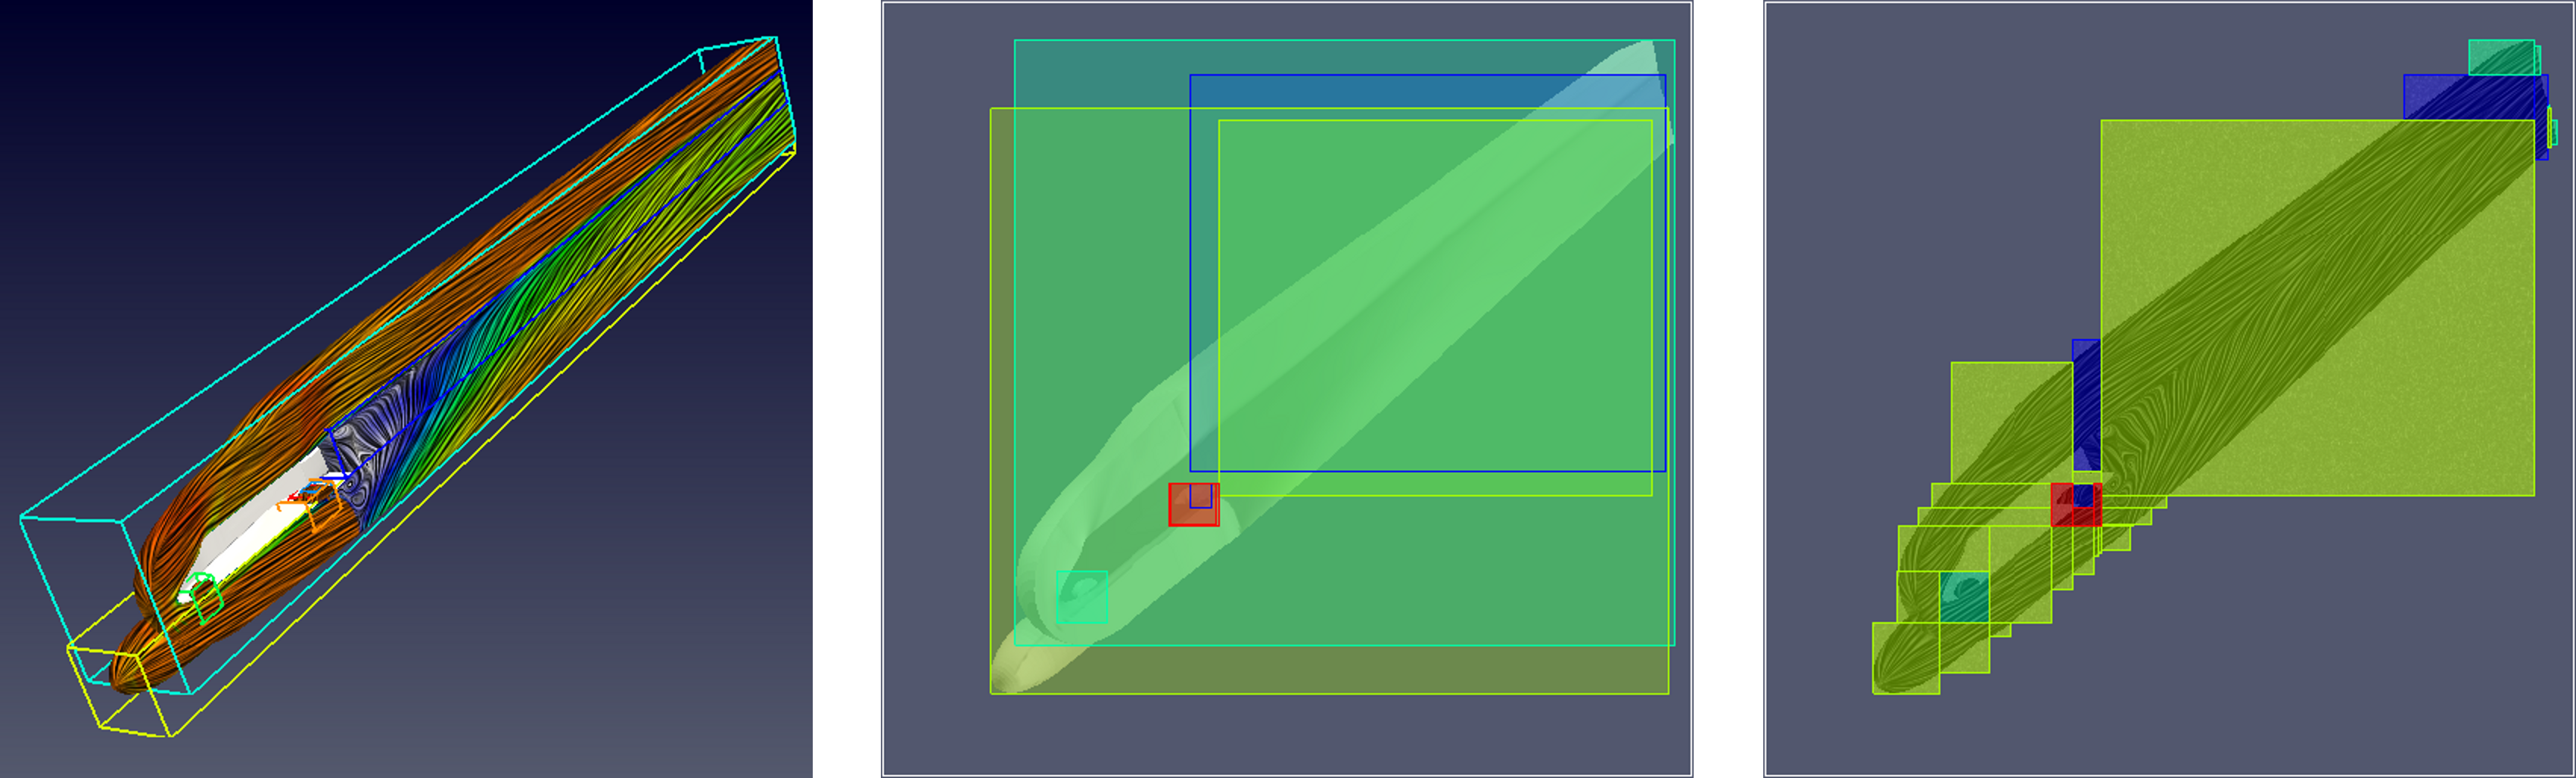
\includegraphics[width=\textwidth]{shuttle-inplace-disj.png}
 % shuttle-inplace-disj.png: 3404x1028 pixel, 72dpi, 120.07x36.26 cm, bb=0 0 3404 1028
 \caption{\small Domain decomposition. The physical space decomposition(left) is transformed into a screen space decomposition(center). Data in overlapping area between processes needs to be exchanged and composited and results in redundant computation. Making the decomposition disjoint(right) eliminates the need to exchange data and redundant computation.}
 \label{fig:decomps}
\end{figure}

In the DMDPSLR setting, a reasonable data distribution for I/O and filter operations can result in highly unbalanced work load during rendering. User applied filtering operations can exacerbate load imbalances. For example slicing operations can leave many processes without any data. The computational resources on the processes without data go unused during rendering. This is usually not a problem as most rendering algorithms are relatively fast. However, the issue of good screen space load balancing is a concern because of the LIC's high computational cost. The communication, compositing, and computational costs of the screen space LIC are a function of the screen space domain decomposition. An additional complication of working in screen space is that work load and domain decomposition are strongly view dependent. 

An illustrative example of some of the issues is shown in figure \ref{fig:decomps}. In the left panel the surface LIC has been computed on a dataset with 7 blocks distributed across 4 processes. Axis aligned bounding boxes for each block have been included and colored by block id for reference. This domain decomposition results in good load balancing during filtering and I/O portions of the visualization pipeline. However, its transformation into screen space results in a large amount of redundant work and high communication costs during rendering of the surface LIC. 

The initial screen space decomposition is obtained by projecting the axis align block bounding boxes into screen space. Each block maps to a screen space extent upon which surface LIC will be computed. We call this the ``in-place'' decomposition. Two issues that impact performance can arise with the in-place decomposition. First, screen space area that contains no data and thus contributes nothing to the result will be included in communication and compositing as vectors are transformed into screen space and in LIC computations. Second, after the transformation of vectors into screen space overlapping regions have the same vector data and as a result will contain identical results and thus the work done on all but one of the overlapping regions is redundant. These issues can be seen in the middle panel of figure \ref{fig:decomps} which shows the decomposition colored by process id. Many of the extents in this decomposition have large areas where with no data and there is a lot of overlapping area that will result in redundant compositing and computation.

To address these inefficiencies we introduced a repartitioning stage into our vector transform which creates a disjoint screen space decomposition by assigning ownership of overlapping regions to one of the processes. To do this we examine the list of screen space extents one by one, from largest to smallest, and subtract from it the other extents. The subtraction operation is defined such that in cases where there is no overlap between the operands, both are unmodified. In the case where the right operand covers the left entirely the left operand is removed. In the case where the operands overlap, the overlapping region is removed from the left operand, spitting it into a number of smaller extents that cover the remaining area while the right operand is unmodified. The results replace the original in our list of extents and the process continues. After the subtraction process the remaining set of extents is disjoint. The set of disjoint extents are then scanned and shrunk to tightly bound the data removing empty areas from subsequent communication, compositing, and computation. A pass is made to merge extents on the same process where they completely share an edge. We call the resulting set of screen space extents the ``disjoint'' decomposition. 

Compared to the in-place decomposition the disjoint decomposition computes LIC once for each pixel and the communication and compositing costs are reduced. Data from overlapping regions is sent to the process owning the region rather than exchanged, reducing the communication by half. The right panel of figure \ref{fig:decomps} shows the disjoint decomposition for our example, where extents are colored by the owning process id.

While computing the disjoint decomposition is fast and can be done independently in parallel doing so is worth while only when there is a significant amount overlap in the original in-place decomposition. There are some common scenarios where there is little or no overlap in the in-place decomposition, for example in 2D datasets or after a 3D dataset has been sliced by a plane. We use a heuristic to automatically switch between the in-place and disjoint decomposition based on an estimate of the communication and compositing cost.

An estimate of the cost to move from one screen space domain decomposition to another is given by:
\begin{equation}
C(S) = \sum\nolimits_{i=1}^{n_p} \sum\nolimits_{j=1}^{n_e(i)} \left[ \sum\nolimits_{p=1,p \neq i}^{n_p} \sum\nolimits_{q=1}^{n_e(p)} \frac{ \textrm{area}(S_{ij} \cap S^{'}_{pq}) }{ \textrm{area}(V) } \right]
\label{eqn:comm-cost}
\end{equation}
where $S$ and $S^{'}$ are sets of screen space extents in the two decompositions, the first index selects process, and the second index selects the specific extent local to that process, $n_p$ is the number of processes, $n_e(i)$ is the number of extents local to process $i$, the $\cap$ operator takes the intersection of two extents yielding an extent which contains the overlapping area, the $area()$ function computes the number of pixels in an extent, $V$ is the extent that covers the screen. The constraint, $p \neq i$ on the first inner sum excludes local extents.

In plain language, equation \ref{eqn:comm-cost} is the ratio of off process overlapping pixels to the total screen size and is proportional to the communication and compositing work required to move between $S$ and $S^{'}$ screen space domain decomposition. Set $S=S^{'}$ and you get an estimate for the cost of compositing $S$ in place, which is the basis for our heuristic. We examine the in-place decomposition in this way to determine when it's worth moving to the disjoint decomposition. $C(S)<=0.3$ selects the in-place domain decomposition, otherwise the disjoint decomposition is chosen.

For the in-place decomposition, shown in the middle panel of figure \ref{fig:decomps}, $C(S)=1.8$ and our heuristic selects the disjoint decomposition. To estimate the savings of communication and compositing work we evaluate $C(S)$ with $S$ the in-place decomposition, shown in the middle panel, and $S^{'}$ the disjoint decomposition, shown in the right panel of figure \ref{fig:decomps}. In this case $C(S)=0.3$, which is a factor of $6$ savings in communication and compositing overhead, in addition to the efficiency gained by computing LIC only once for each pixel and the elimination of many empty pixels from the computation, compared to using the in-place decomposition.

One complication we faced when integrating our algorithm into ParaView is that IceT does not support altering the screen space domain decomposition during rendering. To work around this we added a scatter stage that moves the result back to the in-place decomposition. Because the regions are disjoint this is a simple copy operation implemented with point to point communication. With this additional communication the total communication costs for our algorithm are equal to or less than the in-place strategy. However, compositing costs are reduced by half, LIC computation costs are reduce by at least half on the overlapping area, and communication is spread out potentially reducing congestion.

\begin{figure}
 \centering
 \includegraphics[width=0.75\textwidth]{scaling-datasets-wide.png}\vspace{0.1in}
%  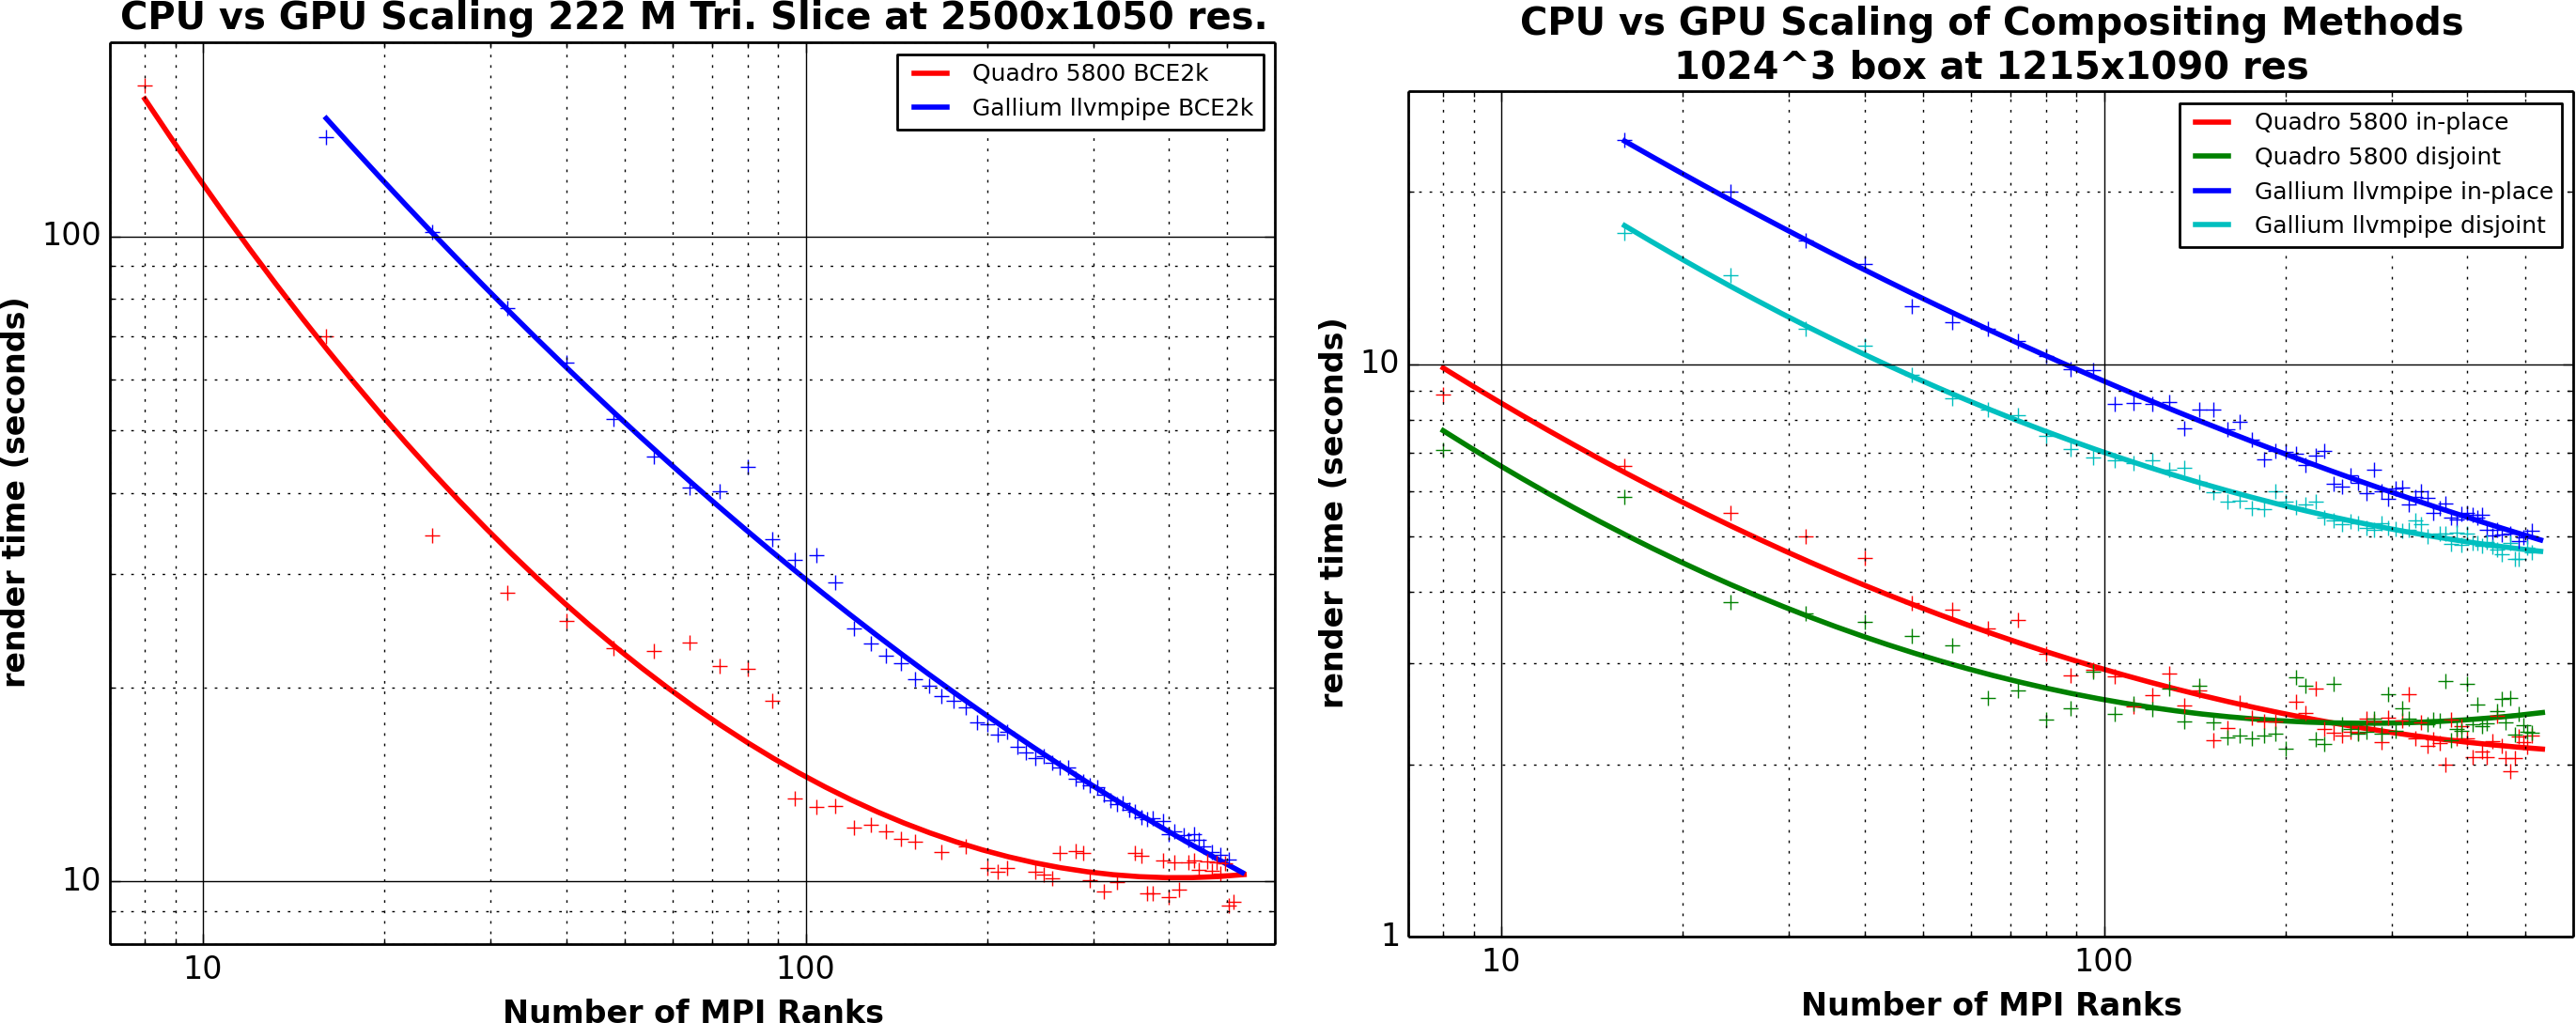
\includegraphics[width=0.9\textwidth]{scaling-gpu.png}
  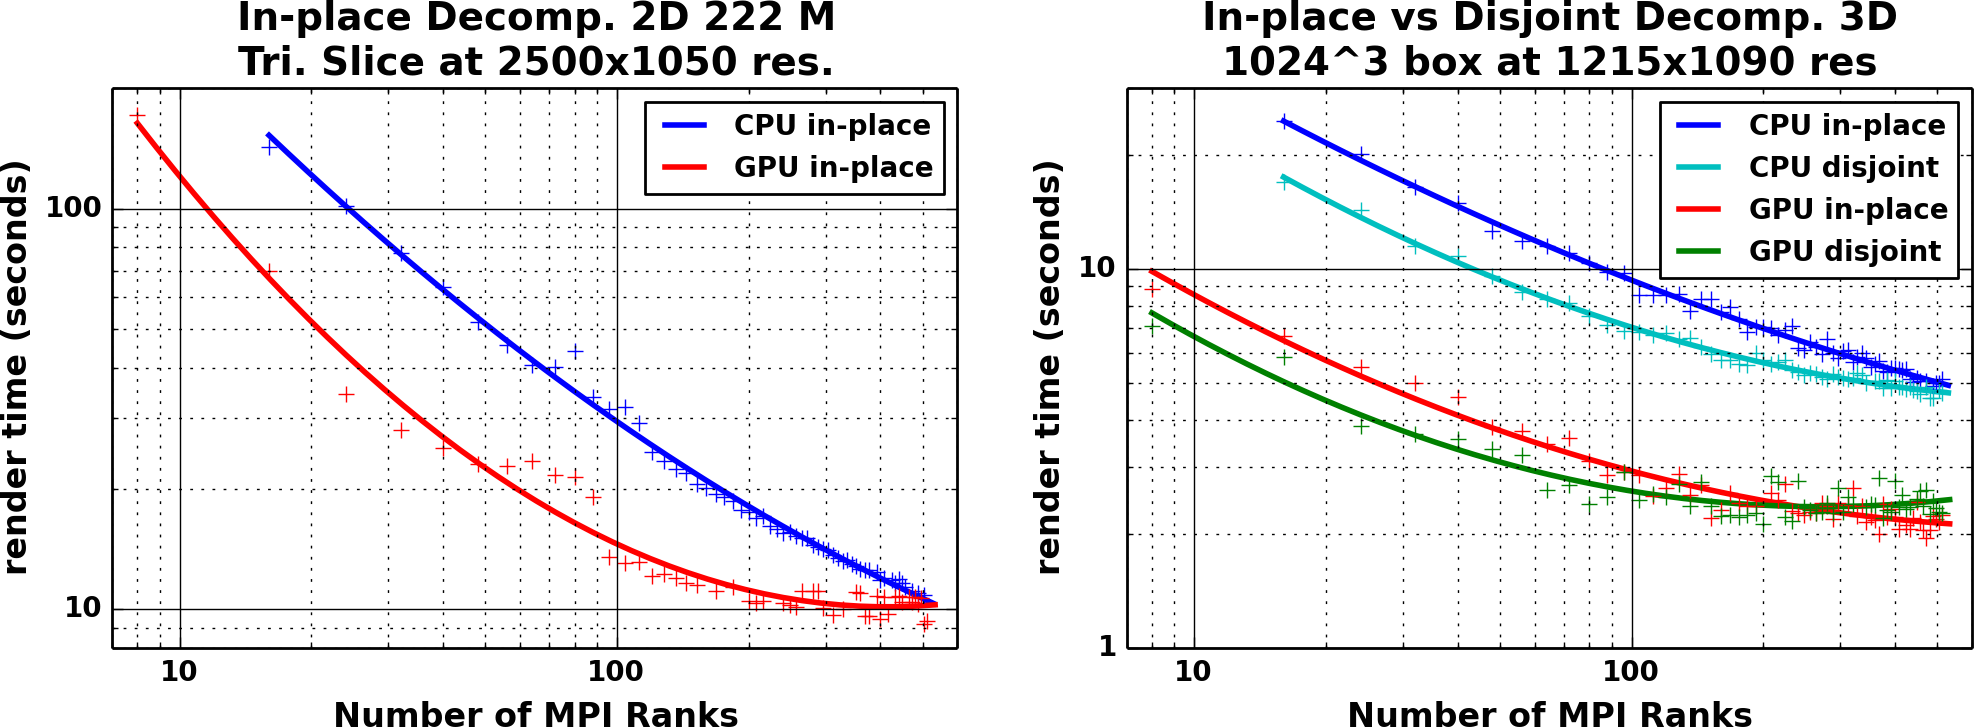
\includegraphics[width=0.9\textwidth]{astronum-2014.png}
 \caption{\small Strong scaling. Top row: Renderings as produced by the test configuration on 2D PIC and 3D MHD simulation of turbulent plasma. Bottom row: Rendering time as a function of number of processes with and without GPUs. Left: Runs with 2D dataset and in-place decomposition. Right: Runs on 3D dataset and in-place and disjoint decompositions.}
 \label{fig:scaling}
\end{figure}

\section{Results}
\subsection{Scaling}
We investigated the strong scaling behavior of our parallel algorithm and compare the in-place and disjoint domain decomposition strategies with and without GPUs. The runs on GPUs were made on TACC's Longhorn cluster where each compute node is equipped with 48GB RAM, two 4 core 2.5GHz Intel E5540 CPUs, two NVIDIA Quadro FX 5800 GPUs, and a QDR 4 GB/sec Infiniband network. Four processes were assigned to each node with two processes assigned to each GPU. The runs made without GPUs were made on NERSC's Cray XC30 Edison I, where each node is equipped with 64GB RAM, two 8 core Intel E5-2670 CPUs, and a Cray Aries 8 GB/sec network. On Edison Mesa 9.2.0 Gallium llvmpipe, a software implementation of OpenGL, was used. Eight processes were assigned to each node each with four rendering threads. This was previously determined to deliver the best performance in single node benchmarks\citep{xsede13}.

The data used in our scaling study came from a 2D PIC simulation of a turbulent plasma computed on a $8192x16384$ grid \citep{pop}, and 3D MHD simulation of a turbulent plasma computed on a $1024x1024x1024$ grid. We set integration, shading, and contrast enhancement parameters for the runs to produce an aesthetic result on a 2560x1600 WQXGA 30" display. Note that about half the number of integration steps were needed for the 3D dataset. The renderings are shown in the top row of figure \ref{fig:scaling}. Counterintuitively the 2D dataset is the more challenging from a rendering perspective. This is because only surface of the 3D dataset, comprised of $12E6$ triangles, is rendered compared with the entirety of the 2D dataset comprised of $222E6$ triangles.

The second row in figure \ref{fig:scaling} shows the strong scaling results with runs made on the 2D data on the left and 3D data on the right. Only the in-place decomposition was used with the 2D data because this decomposition is already disjoint. Both in-place and disjoint decomposition were used with the 3D data in independent runs. For both datasets the in-place decomposition scaled well to high process counts. With the 3D data, moving to the disjoint decomposition resulted in faster rendering but reduced scalability. On average moving to the disjoint decomposition produced a speed up of 22\% for CPUs and 11\% for GPUs. On the GPUs using the disjoint decomposition scaling ended around 200 processes, while on CPUs scaling ended around 512 processes. For the 2D dataset GPU scaling ended around 512 processes. Overall the algorithm scaled less well on GPUs which we attribute in large part to the extra step of transferring data across PCI bus during communication and in small part to the faster and fatter network pipes, and highly optimized MPI implementation on the Cray system. On average GPU's were faster than CPUs by 43\% for the 2D dataset and by 62\% for the 3D dataset.

\subsection{Conclusions and Future Work}
We have parallelized the screen space surface LIC for use in DMDPSLR frameworks, deployed our algorithm in ParaView, and investigated strong scaling behavior on two real world scientific datasets. Our algorithm eliminates redundant communication, compositing, and LIC computation by automatically moving to a disjoint screen space decomposition when appropriate. Perhaps unsurprisingly, we found that while GPUs are faster they face scalability issues at higher process counts which is likely as a consequence of the cost of moving data to and from the GPU. One direction for future work might include investigating strategies minimizing data movement to and from GPU. For example, a purely local contrast enhancement technique would reduce communication and data movement. Another idea for future work is to investigate alternative screen space domain decomposition strategies. For example the disjoint decomposition strategy we used works by eliminating unnecessary communication and computation but does nothing to ensure good load balancing. An alternative strategy could also add load balancing to ensure that each process has roughly the same amount of work. Finally, it would be worth modifying IceT to allow screen space domain decomposition to change during the render so that the scatter stage could be removed. This would further increase the speed up and improve the scalability of the disjoint decomposition.
\vspace{-0.01in}
\bibliography{loring-astronum-2014}

% DMDPSLR
%%%%%%%%%%%%%%%%%%%%%%%%%%%%%%%%%%%%%%%%%%%%%%%%%%%%%%%%%%%%%%%%%%%%%%
% In the DMDPSLR setting, datasets are loaded and distributed across available processes such that individual processes have roughly equivalent amounts of data. Each process may have one or more blocks\footnote{A block may be any type of dataset, including rectilinear, AMR, and unstructured mesh, etc.} of data. Filtering operations are then applied, which can reduce the data to be rendered. Viewing parameters such as camera position, view frustum, and screen resolution are set to achieve the desired result. Rendering occurs locally followed by a global reduction, compositing stage, that combines the results into a single image for display.
% shading
%%%%%%%%%%%%%%%%%%%%%%%%%%%%%%%%%%%%%%%%%%%%%%%%%%%%%%%%%%%%%%%%%%%%%%
% We note in passing that we implemented algorithms for combining pseudocolor plots with the LIC from both \citep{lic} and \citep{surflic} and gave the user the option to select which of these to use at run time. This is encapsulated in figure \ref{fig:pipeline} in the scalar color shader stage.
%
% CE
%%%%%%%%%%%%%%%%%%%%%%%%%%%%%%%%%%%%%%%%%%%%%%%%%%%%%%%%%%%%%%%%%%%%%%
% An unfortunate property of the LIC process is that as the input noise is transformed, through convolution along stream lines, intensities at the low and high tails of the input noise distribution are shifted toward its center resulting in a reduction in dynamic range and contrast in the output. As integration length increases the intensities in the output approach the median noise value. This has two negative consequences. First, contrast in the streaking patterns is reduced which can make them dificult to discrene. Second, when a speduocolor plot is combined with the LIC its colors are modified, and the image is globably darkened, and its dynamic range reduced, which can make variations and patterns in the pseudocolor plot difficult to discern.
% We used a two pass image LIC to counteract these affects \citep{elic}. 
% pipeline detail
%%%%%%%%%%%%%%%%%%%%%%%%%%%%%%%%%%%%%%%%%%%%%%%%%%%%%%%%%%%%%%%%%%%%%%
% The pipeline contains the following stages: lighting computation and vector transformation, followed by gathering and compositing of vectors onto screen space domains with optional screen space re-partitioning, followed by 2 pass image LIC, followed by a scatter that maps the results back onto the original screen space domains when repartition was used in the gather stage, followed by a shading stage that combines LIC with pseudocolor plot with optional color contrast enhancement, and finally a stage that applies depth test and transfers results to to framebuffer for image compositing and presentation on the screen.
% 
% This sub-pipeline is comprised of a masking computation which selects pixels where LIC will be computed based on a user defined masking criteria\footnote{for example $|\vec{V}|<1.e-3$}, followed by the first LIC integration, follwed by a contrast enhancement, followed by edge enhancement stage, follwed by the second LIC pass which convolves the result of the first pass with the vector field, followed by anit-aliasing stage, followed by a second contrast enhancement stage. All of the stages here are optional, save the first LIC pass which is always executed, and the two contrast enhancement stages, which are always are enabled and disabled in conjunction. Aside from the 2 LIC stages, the remaining stages are applications of various image processing techniques that improve the result.
% parallel overview
%
%%%%%%%%%%%%%%%%%%%%%%%%%%%%%%%%%%%%%%%%%%%%%%%%%%%%%%%%%%%%%%%%%%%%%%
% where two or more extents in the screen space decompositong the vectors needs to 
% To ensure correct surface LIC rendering in a DMDPSLR setting we introduced ``gather'' and ``scatter'' stages, and added global all-reduce to compute minimuma nd mxaimum intensities in the contrast enhancement stages. These stages and inter-process comminication are shown in figure \ref{fig:pipeline} where green double arrows denote inter-process communication. The data on each block in the input dataset is transformed into a screen space extent upon which the LIC is computed. The ``gather'' stage moves vector data via projection and depth buffer compositing of overlapping screen space extents into screen space. It also handles guard pixel halo generation and exchanges.
% 
% Overall throughput can sometimes be greatly improved through a redistribution of screen space data that eliminates redundant computation and reduces comminucation costs. This redistribution is automatically chosen using a heuristic that accounts for input data distribution and view parameters. The  gather stage moves data onto the new domain decompositing and the scatter stage moves the result back onto the original. The scatter stage is not generally necessary. In our case to work with Ice-T \citep{icet}, the compositing library used by ParaView, and is only used when the screen space data distribution is modified. 
%
% old abstract
%%%%%%%%%%%%%%%%%%%%%%%%%%%%%%%%%%%%%%%%%%%%%%%%%%%%%%%%%%%%%%%%%%%%%%
% The standard way to visualize streamlines of a vector field is to seed some points and integrate to trace curves that are instantaneously tangent to the velocity vector. Although useful, this approach can be cumbersome when interactively exploring a dataset. For example, the technique is inherently local and unless feature locations are know apriori it's difficult to select an effective set of seed points. An alternative technique called ”line integral convolution” or LIC, which convolves noise with a vector field producing streaking patterns that follow vector field tangents, has the advantage that a very detailed view of the streamlines over the entire computational domain is found in one step without the need to explicitly specify a set of seed points. However, the technique is computationally expensive and the quality of the results are highly data dependent. In the case of screen space LIC on arbitrary surfaces, which is fast enough for interactive use, the results are highly sensitive to a number of run time parameters such as scene lighting, camera position, orientation, screen resolution, and other view related parameters. As a result of these issues the technique often produces low contrast and low dynamic range images, making flow patterns difficult to discern and pseudo-coloring with scalar fields challenging. This work presents a GPGPU screen space surface LIC algorithm specifically tailored for the parallel interactive visualization and exploration of large composite datasets. Interactivity is achieved through an efficient parallel load balancing and compositing algorithm that simultaneously reduces inter-process communication and redundant computation. New shading algorithms that address variability introduced by data dependence and produce high contrast flow patterns and high dynamic range pseudo-coloring across a wide variety of input data and viewing parameters are presented. We show results from the visual analysis of a PIC simulation of turbulence in a hot magnetized plasma.
%
% from homa's paper
%%%%%%%%%%%%%%%%%%%%%%%%%%%%%%%%%%%%%%%%%%%%%%%%%%%%%%%%%%%%%%%%%%%%%%
% The standard way to visualize streamlines of a vector field is to seed some points and integrate to trace curves that are instantaneously tangent to the velocity vector. Although useful, this approach can be cumbersome when interactively exploring a dataset. For example, the technique is inherently local and unless feature locations are know apriori it's difficult to select an effective set of seed points. An alternative technique called ”line integral convolution” or LIC, which convolves noise with a vector field producing streaking patterns that follow vector field tangents, has the advantage that a very detailed view of the streamlines over the entire computational domain is found in one step without the need to explicitly specify a set of seed points. Because the LIC produces a dense representation of the flow field, features of interest can be quickly identified. LIC is often used in conjunction with scalar pseudocoloring. In this case a specialized shader is used to combine the colors with the gray scale LIC image. Optimized implementations, especially data-parallel or GPU based, are very fast making the technique useful for interactive data exploration. The technique was initially developed for use on images\citep{LIC1}, but has since been extended to arbitrary surfaces\citep{LIC2}, and to volumes as well\citep{LIC3}. The algorithm has been ported to the GPU\citep{LIC5} and data-parallel implementations have been developed\citep{LIC4}.
%
% The LIC algorithm of a vector field defined on an image, $I(x,y)$, is given by the following integral over streamline arcs computed from the center of each pixel location, $x,y$.
% \begin{equation}
%  I(x,y) = \frac{\displaystyle \int_{-L}^{L} k(i)N(S_i)di}{\displaystyle \int_{-L}^{L} k(i) di}
% \end{equation}
% where $L$ is the integration length, $N$ generates the noise value at a given location, $S_i$ is a position on a streamline arc centered at $x,y$, $k(i)$ is an approriate convolution kernel, and $I(x,y)$ is the image  pixel at $x,y$. In practice streamline arcs are computed using an RK method over a fixed number of steps, and $L$ may be a constant for all pixels in $I$, or it may be a function of the local vector field. When $L$ is constant the resulting visualization has a uniform look. When $L$ varies as a function of the vector local field the visualzaiton accurately shows relative strengths of flow features. Because the LIC produces a dense representation of the flow field, features of interest can be quickly identified. LIC is often used in conjunction with scalar pseudocoloring. In this case a specialized shader is used to combine the colors with the gray scale LIC image. Optimized implementations, especially data-parallel or GPU based, are very fast making the technique useful for interactive data exploration. An example of image LIC is shown in the left panel of figure \ref{fig:LIC}. The surface LIC technique we use is similar to image based LIC except first vectors are projected onto the surface then into image space where an image LIC algorithm is used to compute LIC\citep{LIC2}. Lit, pseudocolored surface geometry is combined with the image LIC to produce a realistic rendering of the surface geometry. An example of surface LIC on isocontour of density in VPIC plasma simulation is shown in right panel of figure 
% CE details
%%%%%%%%%%%%%%%%%%%%%%%%%%%%%%%%%%%%%%%%%%%%%%%%%%%%%%%%%%%%%%%%%%%%% 
% 
% Pseudocoloring is a common method for visualizing a scalar field on an arbitrary surface. It is often useful to compbine the Surface LIC with a pseudocoloing to analyze the relationship of a scalar paramter in relation to flow features. Two ways in which pseduocolors can be introduced are by a belending or by mapping process. Blending is given by:
% \begin{equation}
% c_{ij} = L_{ij} * I + S_{ij} * (1 - I)
% \label{eqn:color-blend}
% \end{equation}
% Mapping is given by:
% \begin{equation}
% c_{ij} = ( L_{ij} + f ) * S_{ij}
% \label{eqn:color-map}
% \end{equation}
% where the indices $i,j$ identify a specific fragment, $c$ is final RGB value for the combined LIC pseudocolor plot, $L$ is the gray scale intensity of the LIC, $S$ is the RGB pseudocolor, $I$ is a user defined value between $0$ and $1$, and $f$ is user defined biasing parameter, typically 0, that may be used for fine tuning. 
% 
% Both \ref{eqn:color-blend} and \ref{eqn:color-map} have the potential to alter the pseduocolor color. In this regard an unfortunate property of the convolution of gray scale noise is that as integration length increases the resulting gray scale intensities in the LIC, across all pixels, approach the median noise value. The intensities at the low and high tails of the input noise  distribution are shifted toward its center during the convolution. This has two negative consequences. First, as integration length increases contrast in the streaking patterns is reduced. Streaks become difficult to discern. Second, when combining with pseudocoloring this shift in intensities toward the median across the entire result, modifies colors and leads to dull and dark image. Patterns in the pseudocolor plot become difficult to discern.
% 
% We introduced constrast enhancement stages to adress the issue of low contrast LIC streaks, and to reduce the modification and darkening of colors in pseudocolor plots that occurs as a result of combining with LIC. From \ref{eqn:color-map} it can be seen that where the LIC intensity approaches 1 the pseudocolor value is transfered directly at full unmodified intensity and hue. Additionally where the LIC intensity approaches 0, the color is removed being replaced with the dark streak. It's thus desirable to have many full intensity and zero intensity streaks in the LIC. The former preserves the pseudocolor colors while the latter garauntees high contrast streaking patterns.
% 
% We introduce contrast enhancement stages into the pipeline to ensure effictive accurate combiunation with pseducolors and high contrast streaking. Our contrast enhancement stages make use of an image processing technique called histogram stretching\citep{image_processing_text} which remaps intensity distribution across the full range. 
% \begin{equation}
%   L_{ij} = \frac{L_{ij} - m}{M - m}
%   \label{eqn:hist-stretch}
% \end{equation}
% where, the indices $i,j$ identify a specific fragment, $L$ is the gray scale intensity of the LIC, $m$ is the intensity to map to 0, $M$ is intensity to map to 1. The procedure is automated by setting $m$ and $M$ as follows
% \begin{equation}
%   m = min(L) + F_{m} * ( max(L) - min(L) )
% \end{equation}
% \begin{equation}
%   M = max(L) - F_{M} * ( max(L) - min(L) ) 
% \end{equation}
% where, the $min$ and $max$ operations are computed over all fragments, $F_m$ and $F_M$ are optional adjustment factors, typically $0$ unless fine tuning is desired. When $F_m$ or $F_M$ are non-zero, results are clamped to zero and 1, increasing the number of high and low intensity values. The contrast enhancement stages are applied after the first and second pass image LIC stages. While the motiviation for these stages is dervide from \ref{eqn:color-map}, the technique works well with \ref{eqn:color-blend} which also benefits from increased contrast in the LIC streaks. This type of contrast enhancement can also be applied to the resulting combined surface LIC pseudocolor plot. We introduced a color contrasnt enahnacement stage to do so. This stage applies \ref{eqn:hist-stretch} to the lightness channel of the image in HSL color space.
% \begin{figure}
%  \centering
%  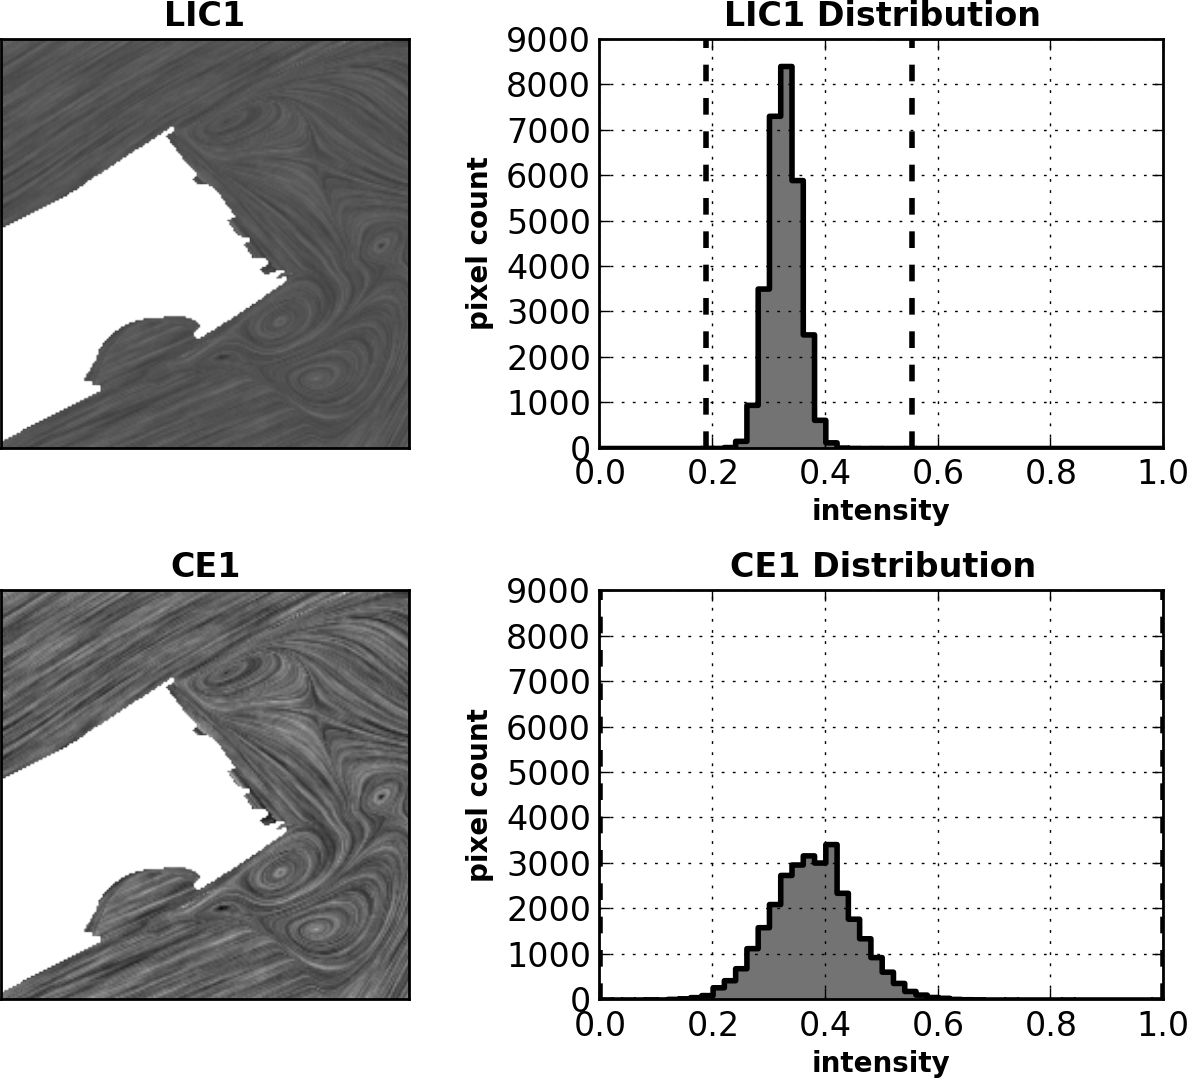
\includegraphics[width=0.3\textwidth]{./gray-ce1-curves.png}
%  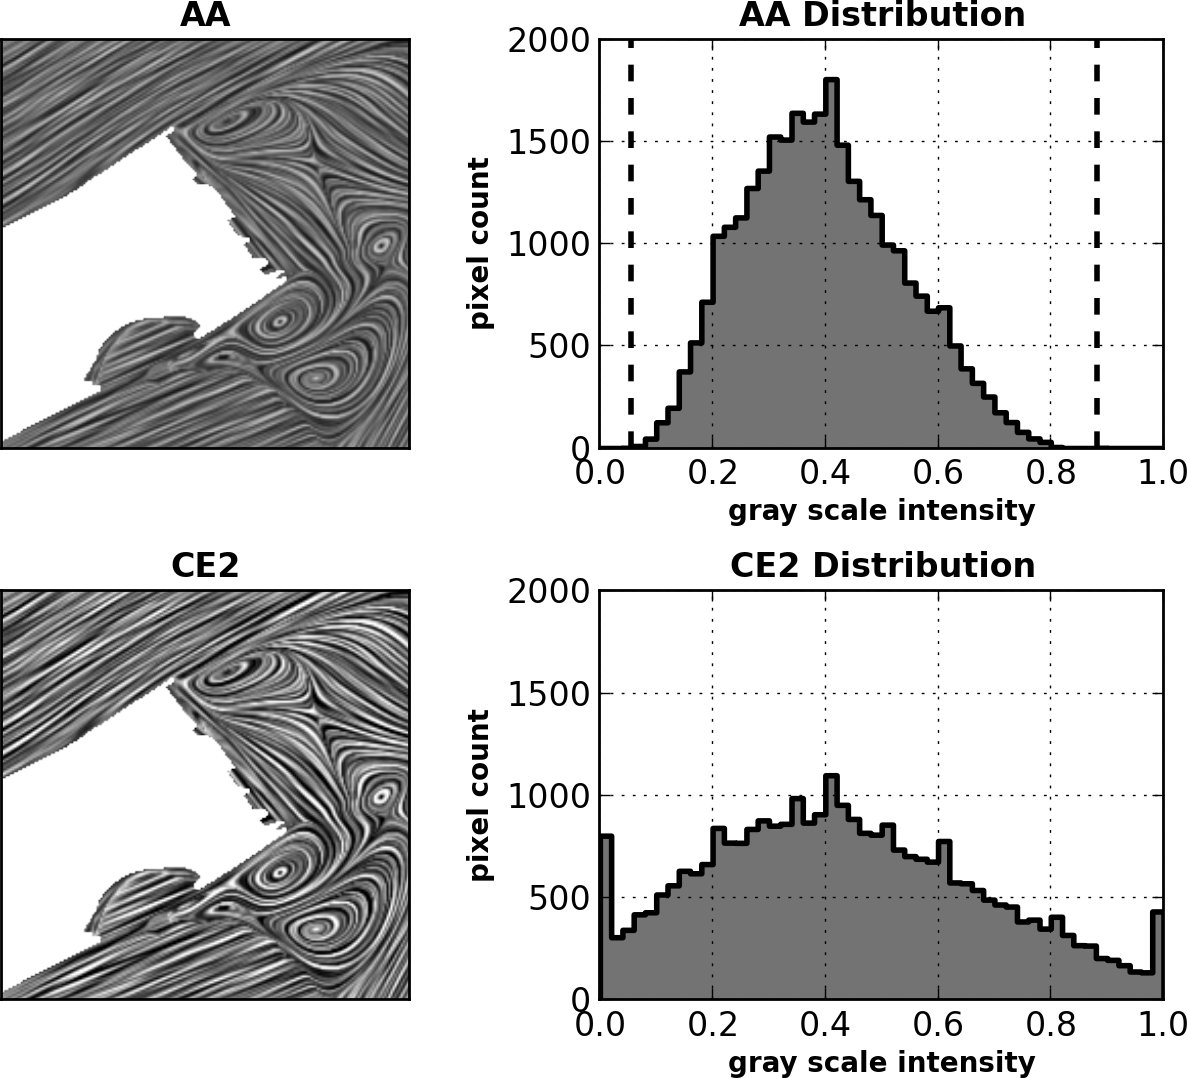
\includegraphics[width=0.3\textwidth]{./gray-ce2-curves.png}
%  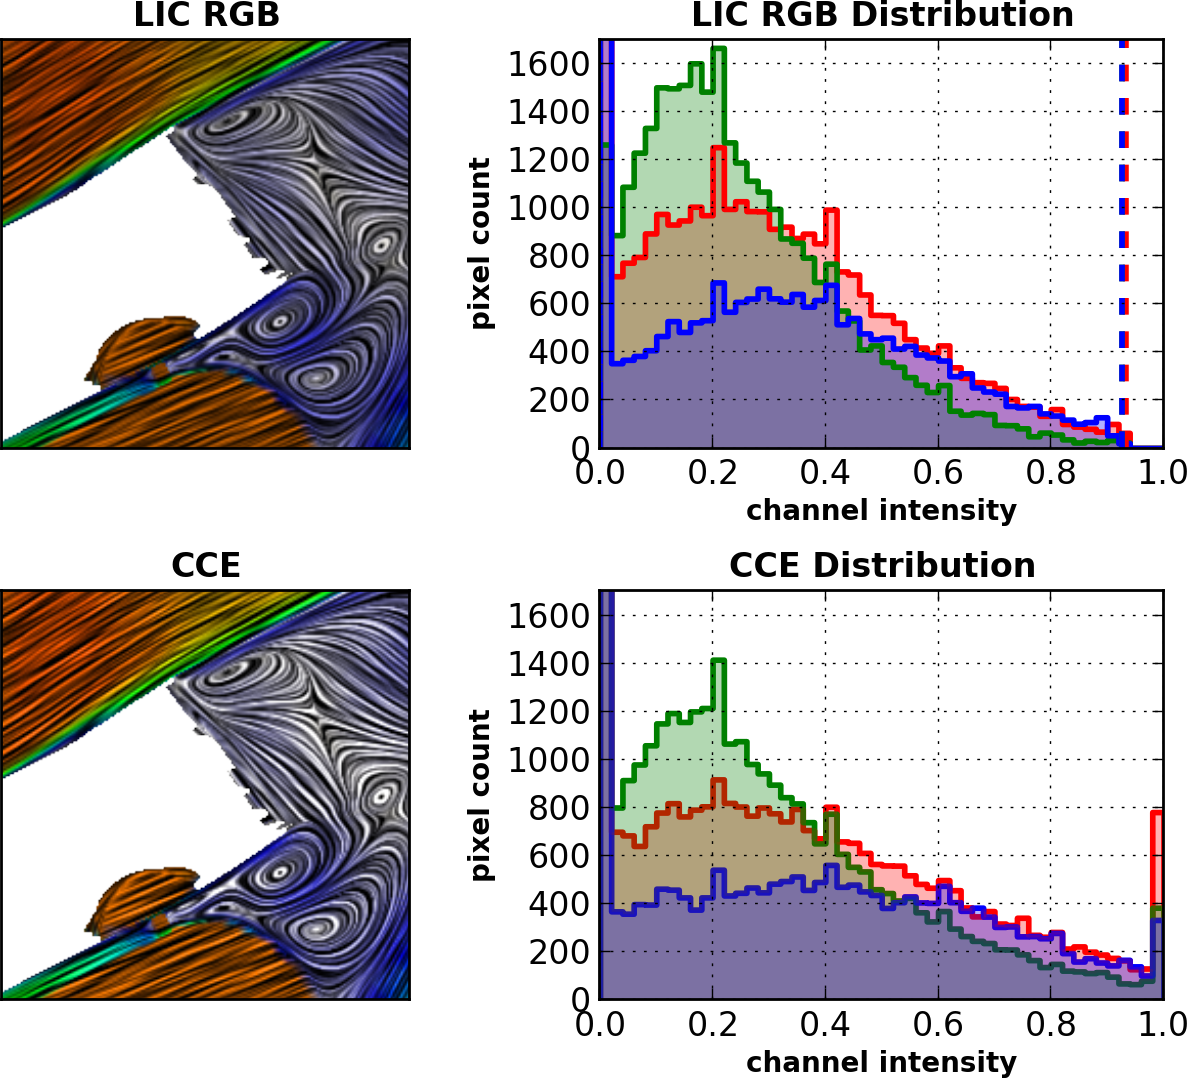
\includegraphics[width=0.3\textwidth]{./color-ce-curves.png}
%  % gray-ce1-curves.png: 1187x1078 pixel, 200dpi, 15.07x13.69 cm, bb=0 0 427 388
%  \caption{ce1}
%  \label{fig:ce1}
% \end{figure}
%
% scalaing result
%%%%%%%%%%%%%%%%%%%%%%%%%%%%%%%%%%%%%%%%%%%%%%%%%%%%%%%%%%%%%%%%%%%%%
% Figure \ref{ce-scaling} shows scaling from 16 to 512 ranks on 2D plasma simulation data computed on a 16384x8192 grid \citep{pop}, \citep{scvs}. The figure shows runs on two vector fields using the settings for a high quality image with and without the contrast enhancement stages. The figure shows that although the new CE feature makes use of MPI\_Allreduce this does not negatively impact scaling. The differences in performance are attributable to the difference in number of integration steps. Typically I've found that to get the look I want I end up using more integration steps when CE is enabled. A sample image from this run is here: http://www.hpcvis.com/vis/vtk-surface-lic-parallelization/kh-new-jaguar-lic-b-woce.png
% 
% Figure \ref{comp-scaling} show scaling from 16 to 512 ranks on a large $1204^3$ MHD turbulence dataset and a comparison of two of the compositing algorithms. The INPLACE option is what you and I had initially discussed on Skype, while the INPLACE\_DISJOINT option ensures that each fragment is computed only once by uniquely assigning ownership of regions of the screen to ranks while leaving the data in-place ie. a rank doesn't take ownership of a fragments it doesn't have data for. For the INPLACE\_DISJOINT approach the compositing communication cost is the same or in some cases less than the INPLACE approach although it's split into two phases(gather and scatter). The figure shows that the INPLACE\_DISJOINT method offers a nice increase in performance. The speed up is larger in the smaller runs because in those runs the screen regions by rank are larger, and this presents a greater opportunity to reduce the number of fragments processed per rank. The following teo plots show this better. The image produced by these runs is here: http://www.hpcvis.com/vis/vtk-surface-lic-parallelization/pr1-lic.png
\end{document}
